%%
% 引言或背景
% 引言是论文正文的开端,应包括毕业论文选题的背景、目的和意义;对国内外研究现状和相关领域中已有的研究成果的简要评述;介绍本项研究工作研究设想、研究方法或实验设计、理论依据或实验基础;涉及范围和预期结果等。要求言简意赅,注意不要与摘要雷同或成为摘要的注解。
% modifier: 黄俊杰(huangjj27, 349373001dc@gmail.com)
% update date: 2017-04-15
%%

\chapter{绪论}
%定义,过去的研究和现在的研究,意义,与图像分割的不同,going deeper

\label{绪论}

\section{选题背景与意义}

% What is the problem
% why is it interesting and important
% Why is it hards, why do naive approaches fails
% why hasn't it been solved before
% what are the key components of my approach and results, also include any specific limitations,do not repeat the abstract
%contribution

Linpack\cite{dongarra1979linpack}基准是国际上最流行的用于测试高性能计算机系统浮点性能的 benchmark,是超级计算机TOP500排名的唯一标准。HPL\cite{HPL}(High Performance Linpack)是第一个标准公开的并行 Linpack测试软件包,由Tennessee大学和Colorado大学共同实现,实现了Linpack基准的MPI版本,可用于大规模集群的Linpack基准测试。

虽然Linpack仍然是衡量超算系统在传统HPC(High Performance Computing) 应用中的性能的可信基准,但现代超算现在正在越来越多地被用于人工智能应用,而不仅仅是数值模拟;大多数AI领域的模型使用混合精度(单精度甚至更低精度浮点格式)计算的方式加速模型推理和训练的效率,而Linpack并不足够衡量计算系统在这一场景中的性能;大量的新基准被提出,始终没有像Linpack一样得到广泛的认可。基于此,Linpack基准和HPL的提出者J. Dongarra对Linpack进行扩展,即 HPL-AI\cite{dongarrahpl},以评估超级计算机在混合精度计算上的性能。

作为近两年提出的新基准,HPL-AI仅给出了单进程的实现作为参考,尚未有公开、通用的多进程、分布式实现。在本文中,我们实现了HPL-AI基准的首个开源的分布式实现\footnote{\url{https://github.com/wu-kan/HPL-AI}},并在包括X86、CUDA、ARM64 在内的多个平台对其正确性、通用性、可扩展性进行了测试。同时,我们将其移植到华为 Atlas 800-9000 AI 训练服务器上,并针对其搭载的国产异构处理器昇腾910进行优化。该移植将交付鹏城实验室,用于对其高性能AI集群``鹏城云脑 II''进行基准测试;同时,我们的工作也为不同平台上的HPL-AI基准测试给出可信参照,对在昇腾平台或其他异构计算平台上的HPC/AI应用优化有很强的指导意义。

\section{国内外相关工作和研究现状}

1979年,高性能计算领域专家J. Dongarra首次提出了Linpack基准\cite{dongarra1979linpack}。该基准通过对高性能计算机在双精度下采用高斯消元法求解一元多次稠密线性代数方程组的计算效率,评价高性能计算机的浮点性能。自基准提出的四十多年以来,Linpack经受住了时间的考验,一直是高性能计算机系统性能的衡量标准,也是一年两次的超算TOP500排名的唯一参照。

因此,Linpack算法的优化被学术界和工业界广泛研究。Y. Saad\cite{saad1986communication}、G. Geist\cite{geist1988lu}、J. Dongarra\cite{dongarra1994scalability,choi1996design}等团队先后提出了并行LU分解算法机及其讨论;S. Toledo\cite{toledo1997locality}、 F. Gustavson\cite{gustavson1997recursion}等团队先后提出了递归LU分解算法及分析;G. Fox\cite{fox1987matrix}、A. Elster\cite{elster1990basic}、J. Dongarra\cite{choi1996design}等团队先后提出了并行矩阵乘法算法设计;M. Heath\cite{heath1988parallel}、G. Li\cite{li1988parallel,li1989new}、R. Bisseling\cite{bisseling1991parallel}等团队先后提出了并行三角矩阵求解算法。

同时,Linpack基准也被包括Intel、IBM、Cray、Fujitsu等在内的硬件厂商移植到各类平台上,见证了摩尔定律下超算性能的指数增长。1993年,洛斯·阿拉莫斯国家实验室的CM-5/1024计算集群以 59.7 GFLOPS 的成绩夺得首个Top500排名第一;1997年,来自桑迪亚国家实验室的``提高战略运算能力计划·红''(ASCI Red)以1.068 TFLOPS的实测性能,标志超算进入TFLOPS的时代;2008年,IBM的``走鹃''(Roadrunner),以微弱优势险胜Cray的``美洲豹''(Jaguar),二者双双达到了每秒千万亿次(PFLOPS)浮点计算能力。

中国在该领域研究中后来居上。2009年,由国防科技大学研制的``天河一号''作为国际上首台采用CPU+GPU异构计算的超算系统,以563.1 TFLOPS的Linpack实测值在Top500榜单中排名第五,证明了GPU异构计算用于大规模Linpack的可行性\cite{wang2011optimizing};2010年,``天河一号''的二期系统``天河一号A''以2.566 PFLOPS的Linpack实测值登顶Top500,标志着中国超算领域达到国际领先水平;2013年,由国防科技大学研制的``天河二号''再次登顶Top500榜单,并连续获得六连冠\cite{liao2014milkyway}。

与此同时,伴随现代人工智能应用的兴起,各类新硬件设计层出不穷。相对于双精度运算单元,它们往往提供更多的低精度运算单元,可使它们在混合精度的场景下获得成倍提升的计算性能和节能效果。这使得研究人员将目光转向使用混合精度加速Linpack求解过程,同时获得与传统Linpack相当的计算精度。2018年,E. Carson等\cite{carson2018accelerating}论证并设计了一种使用三种精度的数值迭代矩阵求解算法;A. Haidar等\cite{haidar2018harnessing}通过混合精度、数值迭代的手段,在特定场景(对角优势矩阵,或特征值恒正的矩阵)下将整个求解过程加速了2.6倍,充分利用了最新NVIDIA GPU中Tensor Core的强半精度算力;2019年,P. Blanchard等\cite{blanchard2020mixed}给出了混合精度下LU分解的舍入误差分析。

基于上述研究,2019年,J. Dongarra提出了HPL-AI基准\cite{dongarrahpl},基于现代算法和当代硬件的融合,统一了传统HPC和现代AI领域的性能标准。HPL-AI的创新处在于,在矩阵求解过程中放弃双精度计算的要求,可以利用已有的和即将推出的AI设备来加速整个求解过程;同时使用数值迭代手段,以恢复在低精度运算中丢失的精度。当NVIDIA在当时全球最快的超级计算机``顶峰''(Summit)上运行HPL-AI基准时,该系统达到了接近0.445 EFLOPS的实测性能,比其在TOP500榜单上的官方性能提升了足足3倍。2020年,来自Fujitsu的``富岳''(Fugaku)作为首台在TOP500中登顶的ARM超算,在HPL-AI基准中将求解速度首次提升至1.42 EFLOPS,相对于其TOP500中的成绩取得3.42倍加速比\cite{DBLP:conf/scala-ws/KudoNII20}。

\begin{wrapfigure}{r}{0.5\linewidth}
    \centering
    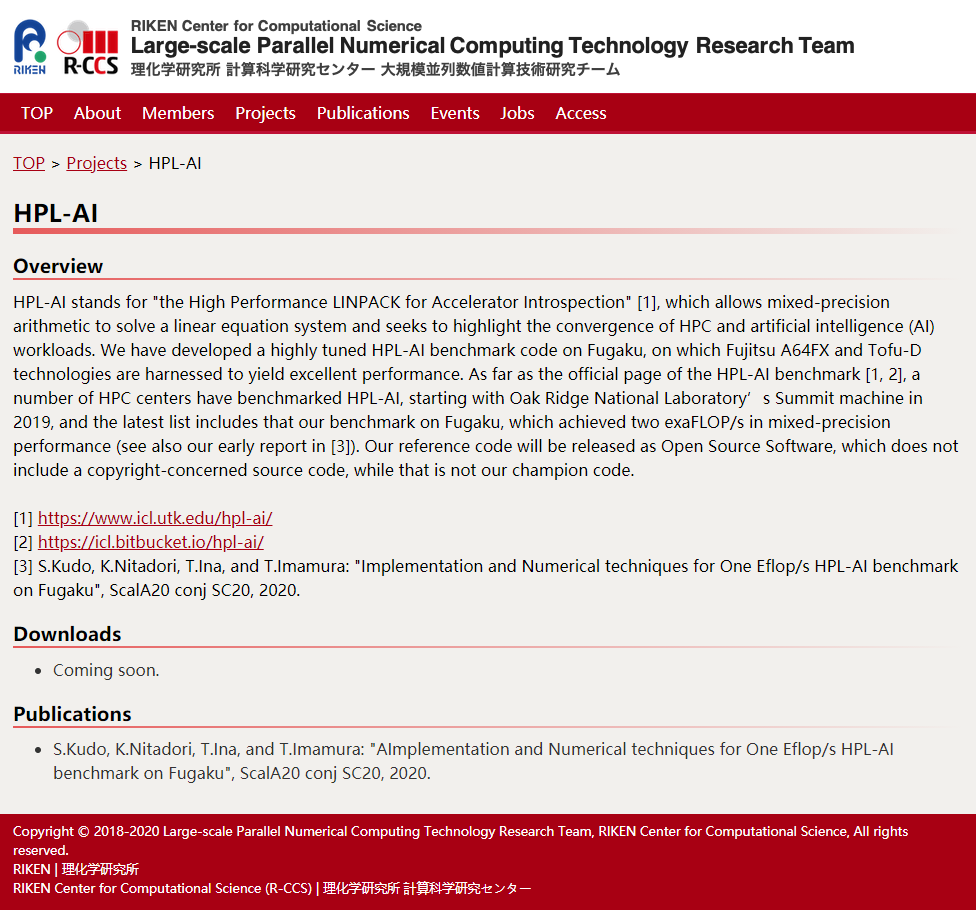
\includegraphics[width=0.5\textwidth]{image/chap01/1}
    \caption{理化学研究所仍未开源}
    \label{理化学研究所仍未开源}
\end{wrapfigure}

当前,已知的HPL-AI实现主要有如下几个版本:

\begin{itemize}

    \item HPL-AI主页提供了一份单进程参考实现\footnote{\url{https://bitbucket.org/icl/hpl-ai/}},但不可用于多进程大规模计算;
    \item NVIDIA在其HPC-Benchmarks镜像包中提供了专用于NVIDIA GPU的HPL-AI-NVIDIA二进制包,但并未开源\footnote{\url{https://ngc.nvidia.com/catalog/containers/nvidia:hpc-benchmarks}};
    \item 理化学研究所宣称将要开源一份HPL-AI实现(并非其用于富岳的调优版本)\footnote{\url{https://www.r-ccs.riken.jp/labs/lpnctrt/projects/hpl-ai/index.html}},但截至{\today}本文正式完稿之时,仍处于未来时态。

\end{itemize}

\section{论文结构与章节安排}

本文共分为五章,各章节内容安排如下:

\autoref{绪论}:绪论。简述本文的选题背景与意义,并介绍了国内外相关工作和研究现状。

\autoref{HPL-AI算法分析与实现}:HPL-AI算法分析与实现。说明了HPL-AI基准的规则,并分析了使用的矩阵构造算法、LU分解算法、数值迭代算法。

\autoref{面向国产异构处理器的移植工作}:面向国产异构处理器的移植工作。分析了昇腾910的硬件架构,并介绍了AscendCL编程模型,并通过实验对使用加速卡的各流程进行Profile,对比了各API和算子的启动开销。基于这些工作得到一个合理的移植方案。

\autoref{实验及分析}:实验及分析。给出了在移植平台及对照平台上软件的测试实验结果,对其正确性、通用性、可扩展性进行验证、分析。

\autoref{总结与展望}:总结与展望。总结了本文的主要成果,并对后续工作进行展望。